% Part 2 chapter carrying "Dark Energy Evolution and the Far Future of an IAM Universe" (Mahaffey, Feb 2026) in its order. Read in full
% 2026-10-02 (609 lines, 50-line ledger). Numbers: docs/verification/scripts/verify_wz_far_future.py. Check: docs/verification/
% observations/WZ_FAR_FUTURE_CHECK.md. Heat-death arguments 2-3 are interpretation (Part 5 closing chapter).
\chapter{The equation of state of the record}\label{ch:darkenergy}

\section*{The place}
The cosmic horizon, at $T_{GH}=\hbar H/2\pi k_B$; the record is $S_{\rm info}$, written by matter as it collapses into structure
(Chapter~\ref{ch:surfaces}). This chapter asks how the energy of that record behaves as the universe expands, and where it ends.

\section{The equation of state}
The informational contribution enters the matter-sector expansion rate,
\begin{equation}H_m^2(a)=H^2(a)+\beta_mE(a)H_0^2,\qquad E(a)=e^{1-1/a},\qquad\beta_m=\Omega_m/2,\label{part2:eq:Hm}\end{equation}
while the photon sector keeps $H(a)$, the $\Lambda$CDM rate. The term behaves as an energy density $\rho_{\rm info}\propto E(a)$. Energy conservation,
$w=-1-\tfrac13\,d\ln\rho/d\ln a$, with $d\ln E/d\ln a=1/a$, gives
\begin{equation}w_{\rm info}(a)=-1-\frac{1}{3a},\qquad w_{\rm info}(1)=-\tfrac43,\end{equation}
with nothing adjusted. \calc\ A density that grows as the universe expands has $w<-1$; this one grows because structure keeps writing.
\begin{itemize}
\item It is phantom at every finite $a$, and $dw/da=1/3a^2>0$: it becomes less phantom with time and tends to $-1$.
\item There is no Big Rip~\cite{CaldwellBigRip2003}. $E(a)$ is bounded by $e$, so $\rho_{\rm info}$ never exceeds $e$ times its present value.
\item At early times $w_{\rm info}$ is strongly negative, but $\rho_{\rm info}\propto E\to0$: at $z=3$ it is $1.1\,\%$ of $\rho_\Lambda$. The
early-time equation of state has nothing to act on, so high-redshift supernovae cannot see it.
\end{itemize}

\section{Two rulers}

\begin{figure}[htbp]\centering
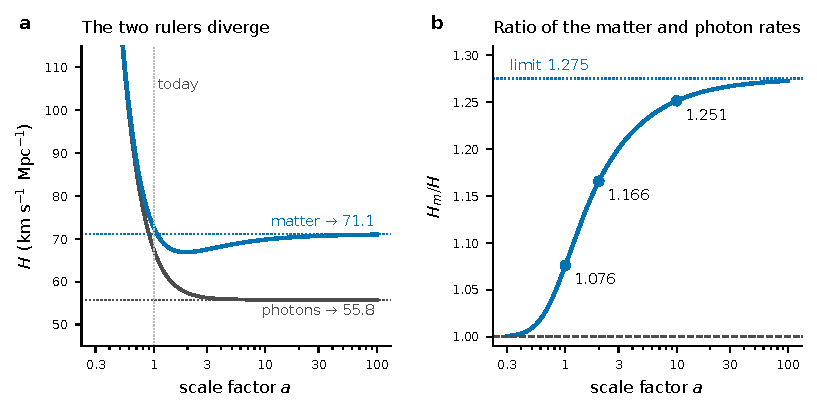
\includegraphics[width=\textwidth]{figures/part2/fig_two_rulers_future.pdf}
\caption{(a) The photon-sector rate $H(a)$ and the matter-sector rate $H_m(a)$ into the future ($H_0=67.4$ for photons): 67.40 and 72.52 today; they settle at $H_0\sqrt{\Omega_\Lambda}=55.8$ and $H_0\sqrt{\Omega_\Lambda+\beta_me}=71.1$\,km\,s$^{-1}$Mpc$^{-1}$. (b) Their ratio: 1.076, 1.166 and 1.251 at $a=1$, 2 and 10, tending to 1.275. \calc}\label{fig:two_rulers_future}
\end{figure}
The photon sector is $\Lambda$CDM, so distances measured with light --- the BAO scale, the CMB acoustic angle, supernova distances on the photon
ruler --- follow $w=-1$. $w_{\rm info}$ belongs to the matter-sector rate \eqref{part2:eq:Hm}. The two rulers diverge as structure grows:
\begin{center}\small\begin{tabular}{lccc}\toprule
$a$ & $H$ (photon) & $H_m$ (matter) & $H_m/H$\\\midrule
1 (today) & 67.40 & 72.52 & 1.076\\ 2 & 57.36 & 66.87 & 1.166\\ 10 & 55.80 & 69.82 & 1.251\\ $\to\infty$ & 55.78 & 71.12 & 1.275\\\bottomrule
\end{tabular}\end{center}
(km\,s$^{-1}$\,Mpc$^{-1}$, with $H_0=67.4$ for the photon sector.) The photon rate settles at $H_0\sqrt{\Omega_\Lambda}=55.8$; the matter rate
settles at $H_0\sqrt{\Omega_\Lambda+\beta_me}=71.1$. \calc\ With the Level~2 photon value $H_0=67.16$ every rate scales by $0.9964$
(the matter-sector rate today becomes $72.26$); the ratios are unchanged.

\paragraph{DESI.} DESI DR2 with the CMB and supernovae~\cite{DESI2025} prefers $w_0=-0.838\pm0.055$, $w_a=-0.62$ (Pantheon+~\cite{Brout2022}), $w_0=-0.667\pm0.088$, $w_a=-1.09$
(Union3~\cite{Rubin2025}) or $w_0=-0.752\pm0.057$, $w_a=-0.86$ (DES Y5~\cite{DESY5SN2024}): above $-1$ today, crossing $-1$ at $z=0.35$--$0.44$. \observed That preference comes from distances ---
the photon ruler --- on which the informational term predicts $w=-1$. Projecting $w_{\rm info}$ onto CPL~\cite{ChevallierPolarski2001,Linder2003} gives $(w_0,w_a)=(-\tfrac43,-\tfrac13)$, $7.6$--$10.2\sigma$
from DESI's $w_0$ \calc; but that projection compares the matter-ruler equation of state with a photon-ruler measurement and is not a test (Chapter~\ref{ch:sectortension}).
The test is the two-ruler
comparison: the expansion history measured with matter (distance ladder, sirens, peculiar velocities) against the history measured with light,
redshift by redshift.

\section{Maturity}

\begin{figure}[htbp]\centering
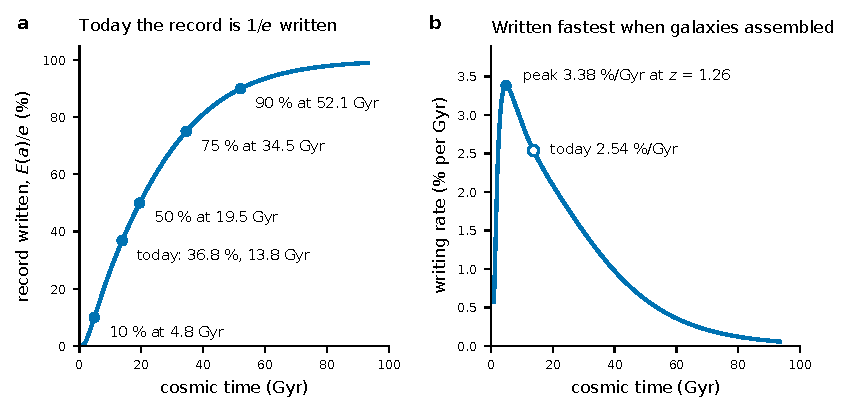
\includegraphics[width=\textwidth]{figures/part2/fig_maturity.pdf}
\caption{(a) The fraction of the eventual record written, $E(a)/e$, against cosmic time (Planck 2018 background): 10\,\% at 4.8\,Gyr, $1/e$ today at 13.8\,Gyr, 50\,\% at 19.5, 75\,\% at 34.5 and 90\,\% at 52.1\,Gyr. (b) The writing rate per unit cosmic time, $dE/dt=HE/a$, as a percentage of the eventual record per Gyr: it peaked at 3.38\,\%\,Gyr$^{-1}$ at $z=1.26$ and is 2.54\,\%\,Gyr$^{-1}$ now. \calc}\label{fig:maturity}
\end{figure}
$E(a)/e$ is the fraction of the eventual record written so far; $a(f)=-1/\ln f$, with ages from the Planck 2018 background~\cite{Planck2018VI}.
\begin{center}\small\begin{tabular}{rrrrr}\toprule
Fraction & $a$ & $z$ & Age (Gyr) & From now\\\midrule
1\,\% & 0.217 & 3.61 & 1.7 & $-12.1$\\ 5\,\% & 0.334 & 2.00 & 3.3 & $-10.5$\\ 10\,\% & 0.434 & 1.30 & 4.8 & $-9.0$\\
20\,\% & 0.621 & 0.61 & 7.8 & $-6.0$\\ 36.8\,\% (today) & 1.000 & 0 & 13.8 & 0\\ 50\,\% & 1.443 & $-0.31$ & 19.5 & $+5.7$\\
75\,\% & 3.476 & $-0.71$ & 34.5 & $+20.7$\\ 90\,\% & 9.491 & $-0.89$ & 52.1 & $+38.3$\\ 99\,\% & 99.50 & $-0.99$ & 93.3 & $+79.5$\\\bottomrule
\end{tabular}\end{center}
Today the record is $1/e=36.8\,\%$ written. How fast it is being written depends on the clock. Per e-fold of expansion, $dE/d\ln a=E/a$ peaks
exactly today, the inflection of $E$ in $\ln a$. Per unit of cosmic time, $dE/dt=HE/a$ peaked at $z=1.26$, about 9 Gyr ago, at $3.4\,\%$ of the
total per Gyr; it is $2.54\,\%$ per Gyr now and falling. \calc

\section{The end state}
The background expands forever, at $H\to55.8$; the far future of the photon sector is the de Sitter state of $\Lambda$CDM. What ends is the writing:
$E\to e$, structure formation stops, and the record on the horizon is complete. The informational term then behaves as a constant, $w\to-1$. \calc

\section{Tests}
The tests of the term --- the two-ruler expansion history $H_m(z)/H(z)$ from \eqref{part2:eq:Hm}, one $E(a)$ in growth and in expansion, and the
falsifier --- are set out in Chapter~\ref{ch:wzfuture}.
